\section{Introduction}
Recently, there has been a great interest in human-robot teaming in civilian (e.g., at factories, hotels, hospitals, homes) and military (e.g., reconnaissance) applications. Communication plays an important role in effective teaming between humans and robots. One way of communication is via natural language, which provides a rich, intuitive, and flexible medium. Accordingly, the grounding problem in the literature addresses the question of how a robot can understand the meaning of a natural language command in the context of its world model (e.g., \cite{g3,dcg}). 
%However, this requires a robot to understand natural language commands  domains including, but not limited to, Robots must be able to understand natural language if they are to efficiently collaborate with humans. In order to achieve this goal, the problem of associating phrase with real-world objects and actions, commonly referred to as the grounding problem, has emerged as a focus of new research in robotics (\textcolor{blue}{REF: G3,DCG, etc.}).

The existing methods to solve the grounding problem make two primary assumptions. First, they assume a fixed set of phrases that can constitute the commands and a fixed set of objects that exist in the world model. Thus, such methods typically fail to reason about unknown phrases or objects that have never been encountered (e.g., in the training process).
Second, these methods often assume that the location of the object being grounded to is known (e.g., the phrases refer to the objects that are currently perceived or localized within a known map).
As a result, a robot using these methods tends to pick the most likely perceived grounding rather than exploring its surroundings.

Note that the aforementioned assumptions do not typically reflect the reality. For example, humans tend to use context-specific lexicons that the general population does not recognize. Moreover, they often refer to objects whose locations may be unknown. To deal with such cases, training a robot to know the meaning of every possible word is infeasible and inefficient. Also, attempting to reason over the space of all possible maps is similarly computationally infeasible.

\begin{figure}[t]
	\centering
	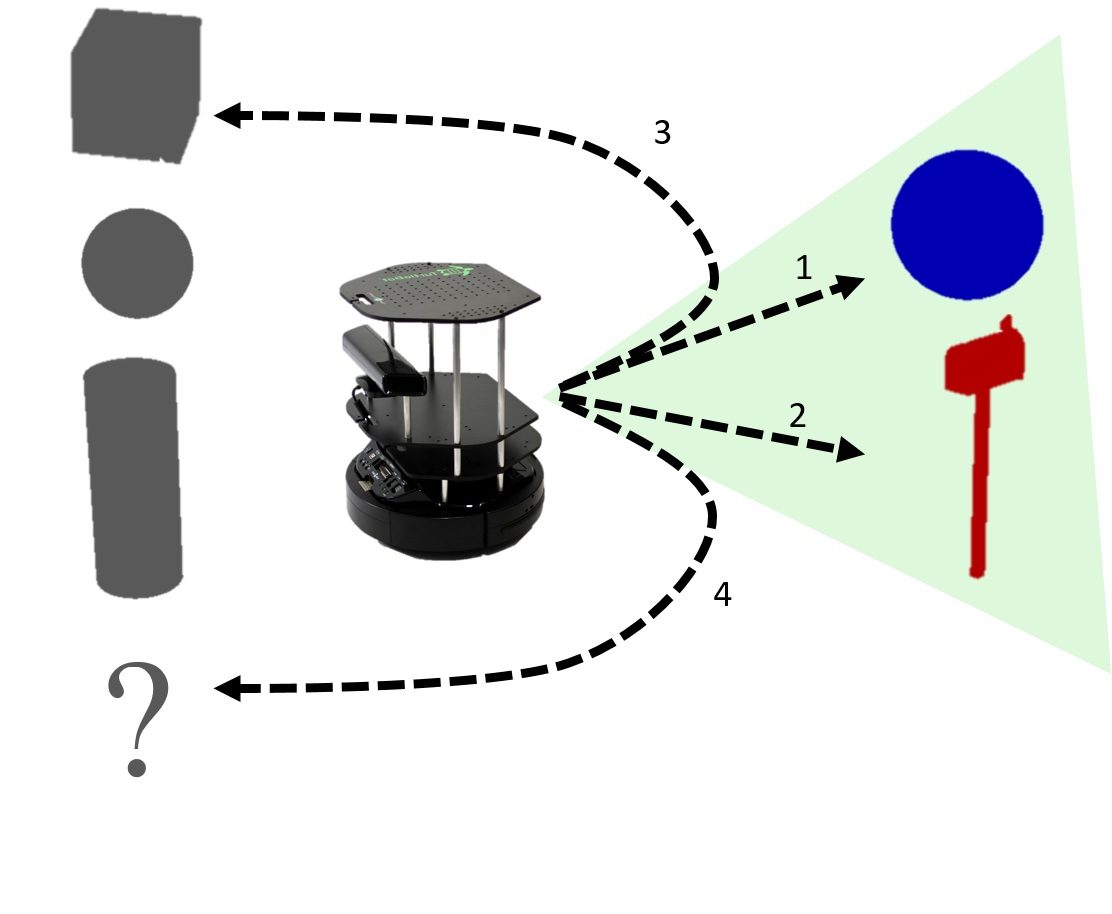
\includegraphics[width=7.1cm]{intro_pic}
	\caption{An illustration of the proposed model DCG-UPUP-Away, which has been trained only with cubes, spheres, and cylinders; and it may ground phrases to known perceived objects (1), unknown perceived objects (2), known hypothesized objects (3), or unknown hypothetical objects (4).}
	\label{fig:intro_pic}
\end{figure}
%To assume that language will be drawn from a fixed set and to assume that language only refers to known, perceived objects is unsafe in the real world.
%Humans regularly draw upon context-specific lexicons that the general population does not recognize; however, training a robot to know every possible meaning of every possible word is infeasible and inefficient.
%At the same time, humans often refer to objects whose locations are fundamentally unknown.
%Attempting to reason over the space of all possible maps, however, is similarly computationally infeasible.

This paper proposes a new model called the Distributed Correspondence Graph - Unknown Phrase, Unknown Percept - Away (DCG-UPUP-Away), which relaxes two aforementioned assumptions by 1) explicitly modeling unknown phrases and unknown percepts, and 2) creating hypothetical objects that can be out of perception.
These two changes yield a model that correctly grounds a large variety of phrases in challenging environments while autonomously learning new words and symbols.
This anecdotal evidence is supported by a simulation study using commands generated by Amazon Mechanical Turk users.
Also, the performance of the proposed model is evaluated via real experiments where a turtlebot is initially trained to recognize a small set of phrases and objects. The results demonstrate that the robot correctly grounds commands approximately 80\% of the time while learning new concepts in an unsupervised manner.

The remainder of this paper is organized as follows:
The preliminaries on probabilistic graphical models used for the grounding problem is introduced in Section~\ref{sec:background}.
The technical approach used in developing the DCG-UPUP-Away model is presented in Section~\ref{sec:technical}.
The model is evaluated in Section~\ref{sec:evaluation}.
Existing research in natural language robotics and human-robot interaction that complements this work are reviewed in Section~\ref{sec:related}. Finally, Sections~\ref{sec:conclusion} concludes the paper by summarizing the contributions and future research.
